\documentclass[tikz, border=10pt]{standalone}
\usepackage{tikz}
\usetikzlibrary{arrows.meta, shapes, positioning}
\usepackage{xcolor}
\definecolor{skyblue}{RGB}{135,206,235}
\tikzset{bigskybluenode/.style={circle, fill=skyblue, draw=black, line width=1pt},smallskybluenode/.style={circle, fill=skyblue, draw=black, line width=0.5pt, minimum size=4pt, inner sep=0pt}}
\definecolor{cyan}{RGB}{0,255,255}
\tikzset{bigcyannode/.style={circle, fill=cyan, draw=black, line width=1pt},smallcyannode/.style={circle, fill=cyan, draw=black, line width=0.5pt, minimum size=4pt, inner sep=0pt}}
\begin{document}
    % Graph for 3 attributes
    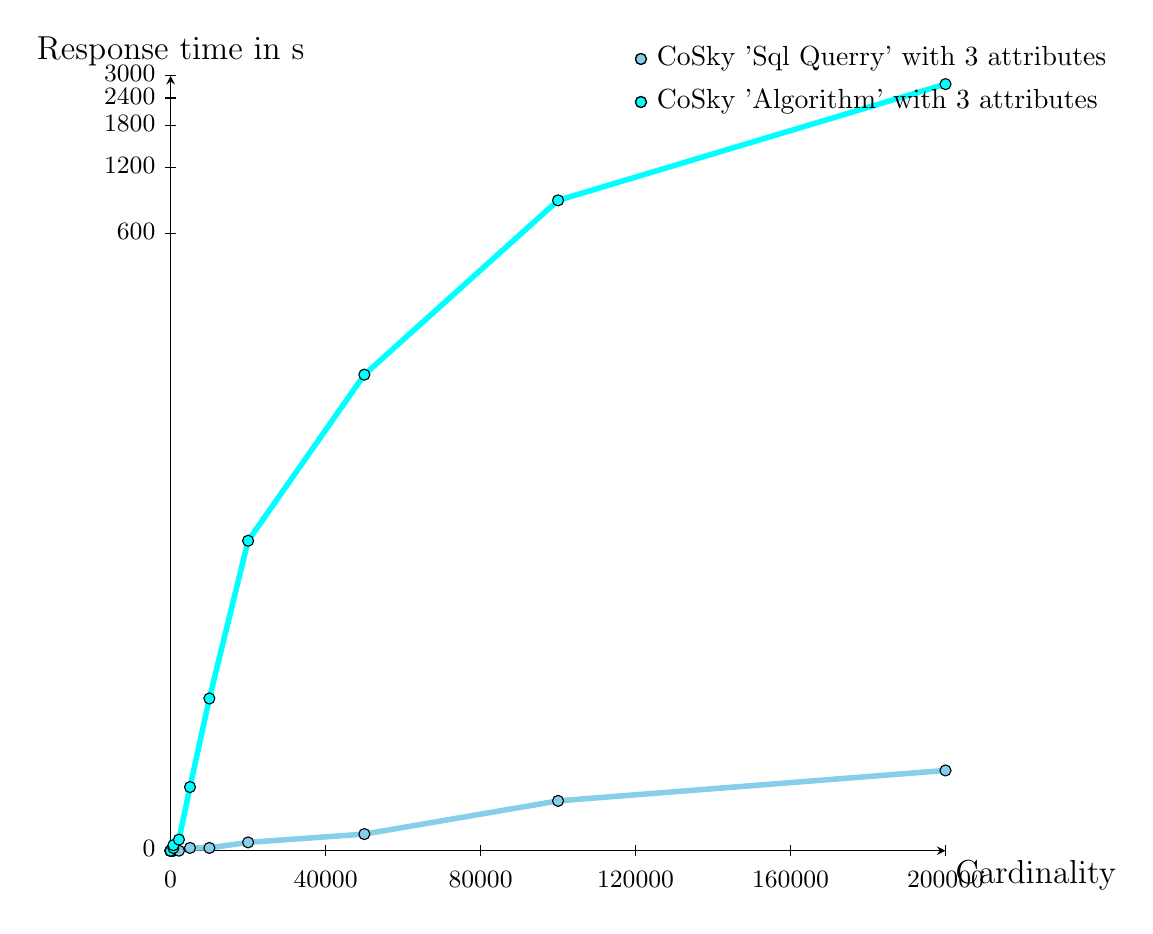
\begin{tikzpicture}[
        line join=bevel,
        bigskybluenode/.style={shape=circle, fill=skyblue, draw=black, line width=1pt},
        bigcyannode/.style={shape=circle, fill=cyan, draw=black, line width=1pt},
        smallskybluenode/.style={circle, fill=skyblue, draw=black, line width=0.5pt, minimum size=4pt, inner sep=0pt},
        smallcyannode/.style={circle, fill=cyan, draw=black, line width=0.5pt, minimum size=4pt, inner sep=0pt}
    ]
        % Axes
        \draw[-stealth] (0pt, 0pt) -- (280pt, 0pt) node[anchor=north west, font=\large] {Cardinality};
        \draw[-stealth] (0pt, 0pt) -- (0pt, 280pt) node[anchor=south, font=\large] {Response time in s};
        % Axis graduation
        \foreach \x/\xtext in {
            0pt/$0$, 
            56pt/$40000$, 
            112pt/$80000$, 
            168pt/$120000$, 
            224pt/$160000$, 
            280pt/$200000$} {
            \draw (\x, 2pt) -- (\x, -2pt) node[below, font=\small] {\xtext\strut};
        }
        \foreach \y/\ytext in {
            0pt/$0$, 
            223pt/$600$, 
            247pt/$1200$, 
            262pt/$1800$, 
            272pt/$2400$, 
            280pt/$3000$} {
            \draw (2pt, \y) -- (-2pt, \y) node[left, font=\small] {\ytext\strut};
        }
        % Lines
        \draw[skyblue, line width=2pt](0pt, 0pt) -- (0pt, 0pt) -- (0pt, 0pt) -- (0pt, 0pt) -- (0pt, 0pt) -- (1pt, 0pt) -- (1pt, 0pt) -- (3pt, 0pt) -- (7pt, 1pt) -- (14pt, 1pt) -- (28pt, 3pt) -- (70pt, 6pt) -- (140pt, 18pt) -- (280pt, 29pt);
        \draw[cyan, line width=2pt](0pt, 0pt) -- (0pt, 0pt) -- (0pt, 0pt) -- (0pt, 0pt) -- (0pt, 0pt) -- (1pt, 1pt) -- (1pt, 2pt) -- (3pt, 4pt) -- (7pt, 23pt) -- (14pt, 55pt) -- (28pt, 112pt) -- (70pt, 172pt) -- (140pt, 235pt) -- (280pt, 277pt);
        % Points
        \filldraw[color=black, fill=skyblue] (0pt, 0pt) circle (2pt);
        \filldraw[color=black, fill=skyblue] (0pt, 0pt) circle (2pt);
        \filldraw[color=black, fill=skyblue] (0pt, 0pt) circle (2pt);
        \filldraw[color=black, fill=skyblue] (0pt, 0pt) circle (2pt);
        \filldraw[color=black, fill=skyblue] (0pt, 0pt) circle (2pt);
        \filldraw[color=black, fill=skyblue] (1pt, 0pt) circle (2pt);
        \filldraw[color=black, fill=skyblue] (1pt, 0pt) circle (2pt);
        \filldraw[color=black, fill=skyblue] (3pt, 0pt) circle (2pt);
        \filldraw[color=black, fill=skyblue] (7pt, 1pt) circle (2pt);
        \filldraw[color=black, fill=skyblue] (14pt, 1pt) circle (2pt);
        \filldraw[color=black, fill=skyblue] (28pt, 3pt) circle (2pt);
        \filldraw[color=black, fill=skyblue] (70pt, 6pt) circle (2pt);
        \filldraw[color=black, fill=skyblue] (140pt, 18pt) circle (2pt);
        \filldraw[color=black, fill=skyblue] (280pt, 29pt) circle (2pt);
        \filldraw[color=black, fill=cyan] (0pt, 0pt) circle (2pt);
        \filldraw[color=black, fill=cyan] (0pt, 0pt) circle (2pt);
        \filldraw[color=black, fill=cyan] (0pt, 0pt) circle (2pt);
        \filldraw[color=black, fill=cyan] (0pt, 0pt) circle (2pt);
        \filldraw[color=black, fill=cyan] (0pt, 0pt) circle (2pt);
        \filldraw[color=black, fill=cyan] (1pt, 1pt) circle (2pt);
        \filldraw[color=black, fill=cyan] (1pt, 2pt) circle (2pt);
        \filldraw[color=black, fill=cyan] (3pt, 4pt) circle (2pt);
        \filldraw[color=black, fill=cyan] (7pt, 23pt) circle (2pt);
        \filldraw[color=black, fill=cyan] (14pt, 55pt) circle (2pt);
        \filldraw[color=black, fill=cyan] (28pt, 112pt) circle (2pt);
        \filldraw[color=black, fill=cyan] (70pt, 172pt) circle (2pt);
        \filldraw[color=black, fill=cyan] (140pt, 235pt) circle (2pt);
        \filldraw[color=black, fill=cyan] (280pt, 277pt) circle (2pt);
        % Caption
        \matrix [below left] at (current bounding box.north east) {
            \node [smallskybluenode, label=right:CoSky 'Sql Querry' with 3 attributes] {}; \\
            \node [smallcyannode, label=right:CoSky 'Algorithm' with 3 attributes] {}; \\
        };
    \end{tikzpicture}
    % Graph for 6 attributes
    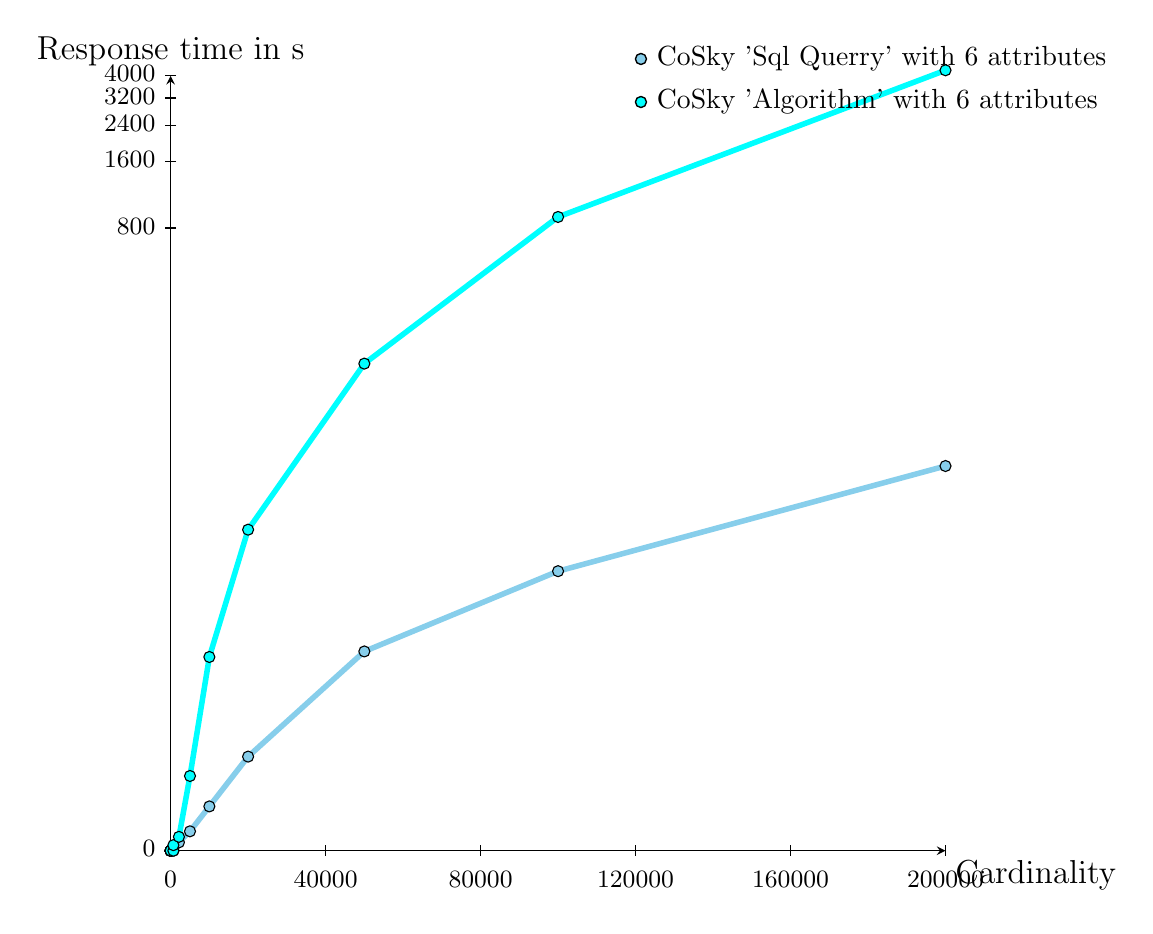
\begin{tikzpicture}[
        line join=bevel,
        bigskybluenode/.style={shape=circle, fill=skyblue, draw=black, line width=1pt},
        bigcyannode/.style={shape=circle, fill=cyan, draw=black, line width=1pt},
        smallskybluenode/.style={circle, fill=skyblue, draw=black, line width=0.5pt, minimum size=4pt, inner sep=0pt},
        smallcyannode/.style={circle, fill=cyan, draw=black, line width=0.5pt, minimum size=4pt, inner sep=0pt}
    ]
        % Axes
        \draw[-stealth] (0pt, 0pt) -- (280pt, 0pt) node[anchor=north west, font=\large] {Cardinality};
        \draw[-stealth] (0pt, 0pt) -- (0pt, 280pt) node[anchor=south, font=\large] {Response time in s};
        % Axis graduation
        \foreach \x/\xtext in {
            0pt/$0$, 
            56pt/$40000$, 
            112pt/$80000$, 
            168pt/$120000$, 
            224pt/$160000$, 
            280pt/$200000$} {
            \draw (\x, 2pt) -- (\x, -2pt) node[below, font=\small] {\xtext\strut};
        }
        \foreach \y/\ytext in {
            0pt/$0$, 
            225pt/$800$, 
            249pt/$1600$, 
            262pt/$2400$, 
            272pt/$3200$, 
            280pt/$4000$} {
            \draw (2pt, \y) -- (-2pt, \y) node[left, font=\small] {\ytext\strut};
        }
        % Lines
        \draw[skyblue, line width=2pt](0pt, 0pt) -- (0pt, 0pt) -- (0pt, 0pt) -- (0pt, 0pt) -- (0pt, 0pt) -- (1pt, 0pt) -- (1pt, 1pt) -- (3pt, 3pt) -- (7pt, 7pt) -- (14pt, 16pt) -- (28pt, 34pt) -- (70pt, 72pt) -- (140pt, 101pt) -- (280pt, 139pt);
        \draw[cyan, line width=2pt](0pt, 0pt) -- (0pt, 0pt) -- (0pt, 0pt) -- (0pt, 0pt) -- (0pt, 0pt) -- (1pt, 0pt) -- (1pt, 2pt) -- (3pt, 5pt) -- (7pt, 27pt) -- (14pt, 70pt) -- (28pt, 116pt) -- (70pt, 176pt) -- (140pt, 229pt) -- (280pt, 282pt);
        % Points
        \filldraw[color=black, fill=skyblue] (0pt, 0pt) circle (2pt);
        \filldraw[color=black, fill=skyblue] (0pt, 0pt) circle (2pt);
        \filldraw[color=black, fill=skyblue] (0pt, 0pt) circle (2pt);
        \filldraw[color=black, fill=skyblue] (0pt, 0pt) circle (2pt);
        \filldraw[color=black, fill=skyblue] (0pt, 0pt) circle (2pt);
        \filldraw[color=black, fill=skyblue] (1pt, 0pt) circle (2pt);
        \filldraw[color=black, fill=skyblue] (1pt, 1pt) circle (2pt);
        \filldraw[color=black, fill=skyblue] (3pt, 3pt) circle (2pt);
        \filldraw[color=black, fill=skyblue] (7pt, 7pt) circle (2pt);
        \filldraw[color=black, fill=skyblue] (14pt, 16pt) circle (2pt);
        \filldraw[color=black, fill=skyblue] (28pt, 34pt) circle (2pt);
        \filldraw[color=black, fill=skyblue] (70pt, 72pt) circle (2pt);
        \filldraw[color=black, fill=skyblue] (140pt, 101pt) circle (2pt);
        \filldraw[color=black, fill=skyblue] (280pt, 139pt) circle (2pt);
        \filldraw[color=black, fill=cyan] (0pt, 0pt) circle (2pt);
        \filldraw[color=black, fill=cyan] (0pt, 0pt) circle (2pt);
        \filldraw[color=black, fill=cyan] (0pt, 0pt) circle (2pt);
        \filldraw[color=black, fill=cyan] (0pt, 0pt) circle (2pt);
        \filldraw[color=black, fill=cyan] (0pt, 0pt) circle (2pt);
        \filldraw[color=black, fill=cyan] (1pt, 0pt) circle (2pt);
        \filldraw[color=black, fill=cyan] (1pt, 2pt) circle (2pt);
        \filldraw[color=black, fill=cyan] (3pt, 5pt) circle (2pt);
        \filldraw[color=black, fill=cyan] (7pt, 27pt) circle (2pt);
        \filldraw[color=black, fill=cyan] (14pt, 70pt) circle (2pt);
        \filldraw[color=black, fill=cyan] (28pt, 116pt) circle (2pt);
        \filldraw[color=black, fill=cyan] (70pt, 176pt) circle (2pt);
        \filldraw[color=black, fill=cyan] (140pt, 229pt) circle (2pt);
        \filldraw[color=black, fill=cyan] (280pt, 282pt) circle (2pt);
        % Caption
        \matrix [below left] at (current bounding box.north east) {
            \node [smallskybluenode, label=right:CoSky 'Sql Querry' with 6 attributes] {}; \\
            \node [smallcyannode, label=right:CoSky 'Algorithm' with 6 attributes] {}; \\
        };
    \end{tikzpicture}
    % Graph for 9 attributes
    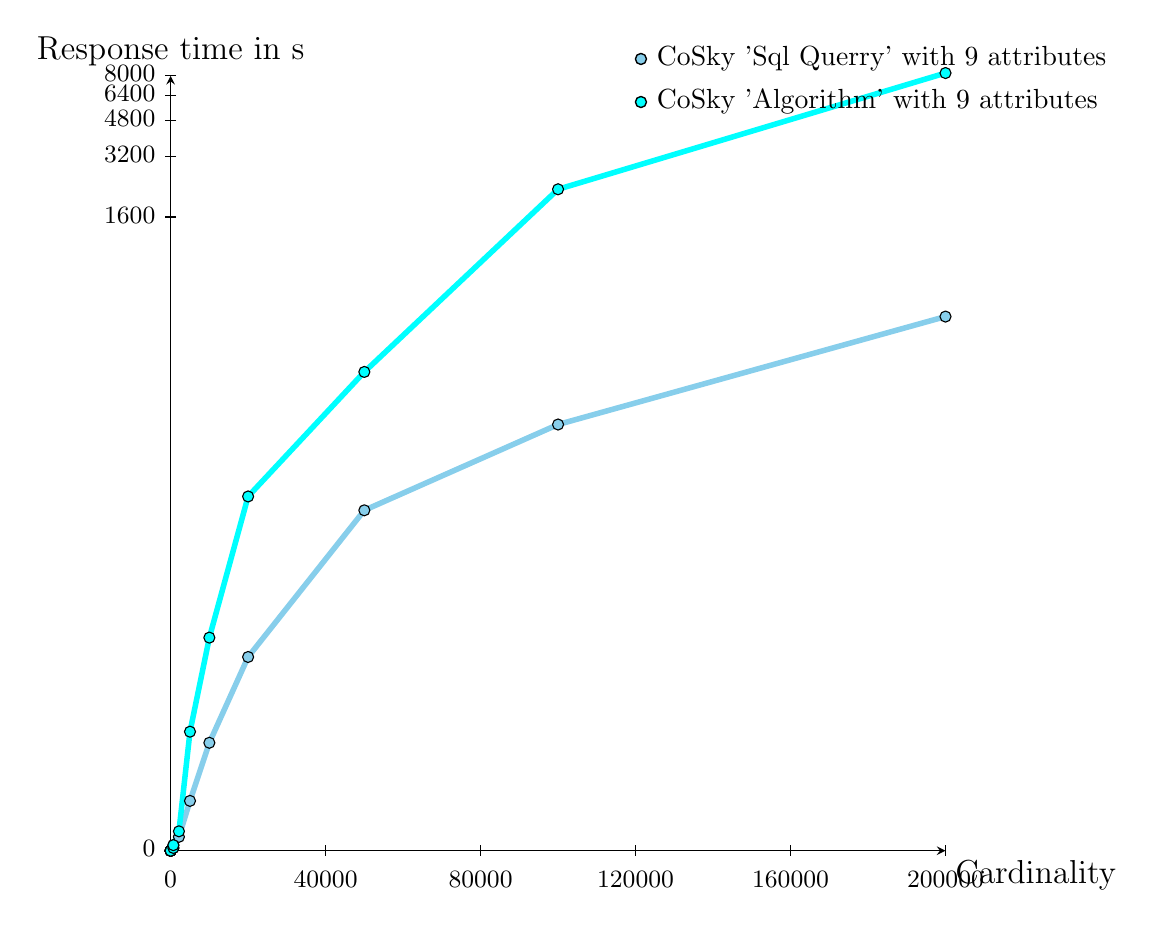
\begin{tikzpicture}[
        line join=bevel,
        bigskybluenode/.style={shape=circle, fill=skyblue, draw=black, line width=1pt},
        bigcyannode/.style={shape=circle, fill=cyan, draw=black, line width=1pt},
        smallskybluenode/.style={circle, fill=skyblue, draw=black, line width=0.5pt, minimum size=4pt, inner sep=0pt},
        smallcyannode/.style={circle, fill=cyan, draw=black, line width=0.5pt, minimum size=4pt, inner sep=0pt}
    ]
        % Axes
        \draw[-stealth] (0pt, 0pt) -- (280pt, 0pt) node[anchor=north west, font=\large] {Cardinality};
        \draw[-stealth] (0pt, 0pt) -- (0pt, 280pt) node[anchor=south, font=\large] {Response time in s};
        % Axis graduation
        \foreach \x/\xtext in {
            0pt/$0$, 
            56pt/$40000$, 
            112pt/$80000$, 
            168pt/$120000$, 
            224pt/$160000$, 
            280pt/$200000$} {
            \draw (\x, 2pt) -- (\x, -2pt) node[below, font=\small] {\xtext\strut};
        }
        \foreach \y/\ytext in {
            0pt/$0$, 
            229pt/$1600$, 
            251pt/$3200$, 
            264pt/$4800$, 
            273pt/$6400$, 
            280pt/$8000$} {
            \draw (2pt, \y) -- (-2pt, \y) node[left, font=\small] {\ytext\strut};
        }
        % Lines
        \draw[skyblue, line width=2pt](0pt, 0pt) -- (0pt, 0pt) -- (0pt, 0pt) -- (0pt, 0pt) -- (0pt, 0pt) -- (1pt, 1pt) -- (1pt, 2pt) -- (3pt, 5pt) -- (7pt, 18pt) -- (14pt, 39pt) -- (28pt, 70pt) -- (70pt, 123pt) -- (140pt, 154pt) -- (280pt, 193pt);
        \draw[cyan, line width=2pt](0pt, 0pt) -- (0pt, 0pt) -- (0pt, 0pt) -- (0pt, 0pt) -- (0pt, 0pt) -- (1pt, 1pt) -- (1pt, 2pt) -- (3pt, 7pt) -- (7pt, 43pt) -- (14pt, 77pt) -- (28pt, 128pt) -- (70pt, 173pt) -- (140pt, 239pt) -- (280pt, 281pt);
        % Points
        \filldraw[color=black, fill=skyblue] (0pt, 0pt) circle (2pt);
        \filldraw[color=black, fill=skyblue] (0pt, 0pt) circle (2pt);
        \filldraw[color=black, fill=skyblue] (0pt, 0pt) circle (2pt);
        \filldraw[color=black, fill=skyblue] (0pt, 0pt) circle (2pt);
        \filldraw[color=black, fill=skyblue] (0pt, 0pt) circle (2pt);
        \filldraw[color=black, fill=skyblue] (1pt, 1pt) circle (2pt);
        \filldraw[color=black, fill=skyblue] (1pt, 2pt) circle (2pt);
        \filldraw[color=black, fill=skyblue] (3pt, 5pt) circle (2pt);
        \filldraw[color=black, fill=skyblue] (7pt, 18pt) circle (2pt);
        \filldraw[color=black, fill=skyblue] (14pt, 39pt) circle (2pt);
        \filldraw[color=black, fill=skyblue] (28pt, 70pt) circle (2pt);
        \filldraw[color=black, fill=skyblue] (70pt, 123pt) circle (2pt);
        \filldraw[color=black, fill=skyblue] (140pt, 154pt) circle (2pt);
        \filldraw[color=black, fill=skyblue] (280pt, 193pt) circle (2pt);
        \filldraw[color=black, fill=cyan] (0pt, 0pt) circle (2pt);
        \filldraw[color=black, fill=cyan] (0pt, 0pt) circle (2pt);
        \filldraw[color=black, fill=cyan] (0pt, 0pt) circle (2pt);
        \filldraw[color=black, fill=cyan] (0pt, 0pt) circle (2pt);
        \filldraw[color=black, fill=cyan] (0pt, 0pt) circle (2pt);
        \filldraw[color=black, fill=cyan] (1pt, 1pt) circle (2pt);
        \filldraw[color=black, fill=cyan] (1pt, 2pt) circle (2pt);
        \filldraw[color=black, fill=cyan] (3pt, 7pt) circle (2pt);
        \filldraw[color=black, fill=cyan] (7pt, 43pt) circle (2pt);
        \filldraw[color=black, fill=cyan] (14pt, 77pt) circle (2pt);
        \filldraw[color=black, fill=cyan] (28pt, 128pt) circle (2pt);
        \filldraw[color=black, fill=cyan] (70pt, 173pt) circle (2pt);
        \filldraw[color=black, fill=cyan] (140pt, 239pt) circle (2pt);
        \filldraw[color=black, fill=cyan] (280pt, 281pt) circle (2pt);
        % Caption
        \matrix [below left] at (current bounding box.north east) {
            \node [smallskybluenode, label=right:CoSky 'Sql Querry' with 9 attributes] {}; \\
            \node [smallcyannode, label=right:CoSky 'Algorithm' with 9 attributes] {}; \\
        };
    \end{tikzpicture}
\end{document}